\chapter{Strictly Sinusoidal Trajectories}
\section{Strictly Sinusoidal Trajectories}
\begin{dfn}
	   	A strictly sinusoidal trajectory for the equation  $\dot{x}(t)=\tilde{A}x$ which satisfies $\ddot{x}_i = -x_i$ and $x_i \neq 0$ for all $i$.
\end{dfn}
\begin{lem}
	Suppose $A$ is irreducible, all 2-cycles in $SD(A)$ are positive, and $SD(A)$ contains no $k$-cycle for $k > 2$. Then there exist $\tilde{A} \in Q(A)$ and sinusoidal $x$ solving $\dot{x} = \tilde{A}x$.
\end{lem}

\begin{proof}
	 When all 2-cycles in $SD(A)$ are positive, it implies that for every pair of nodes $i$ and $j$ in the signed digraph with $i \neq j$, the product of the corresponding entries $a_{ij}$ and $a_{ji}$ in $A$ is positive, i.e., $\lambda_i a_{ij} = \lambda_j a_{ji}$ for some positive constants $\lambda_i$ and $\lambda_j$.
	
	As a result, the matrix formed by scaling the entries of $A$ by $\lambda_i^{1/2}$ and $\lambda_j^{-1/2}$ is symmetric and the symmetric matrix has only real eigenvalues. Since $A$ is diagonally similar to this symmetric matrix, it also has only real eigenvalues.
	
	Furthermore, because $A$ has only real eigenvalues, it cannot support a sinusoidal trajectory since sinusoidal functions have purely imaginary eigenvalues.
	
	Therefore, under the given conditions on $SD(A)$, the existence of $\tilde{A}$ and a sinusoidal trajectory $x$ satisfying $\dot{x} = \tilde{A}x$ is not possible.
	
\end{proof}

\begin{lem}
	Suppose $A$ is irreducible and $SD(A)$ has no 1-cycle or $k$-cycle, $k > 2$, but at least one negative 2-cycle. Then there exist $\tilde{A} \in Q(A)$ and strictly sinusoidal $x$ solving $\dot{x} = \tilde{A}x$.
\end{lem}

\begin{proof}
	We will prove above lemma in a constructive approach.Therefore, suppose signed digraph $SD(A)$ contains a negative 2-cycle. The question of existence is resolved by showing that it is always possible to attach straight chains to any subsystem with strictly sinusoidal nodes. In fact, only $\pm\sin t$ and $\pm\cos t$ are required as node values and the entries of $\tilde{A}$ are specified and modified as needed. 
	We will illustrate this with an example, attaching a straight chain to a subsystem  with node set $\{2,3,\ldots, p\}$ with strictly sinusoidal node at node 1. Let's say node 1 has the value $\sin t$. The idea is illustrated in Figure 3.1. We tentatively assign node $p$ the value $\cos t$ if $p$ is even, or $\sin t$ if $p$ is odd. Then we'll set $|\tilde{a}_{p,p-1}| = 1$, so that the sign of $\tilde{a}_{p,p-1}$ determines whether node $p-1$ in $\dot{x} = \tilde{A}x$ is $\pm\dot{x_p}$, that is $\pm \sin t$ if $p$ is even, $\pm \cos t$ if $p$ is odd.
	
	
	Consider the equation at row $p-1$. Specifying either $|\tilde{a}_{p-1,p-2}| = |\tilde{a}_{p-1,p-2}| = 1/2$ or $|\tilde{a}_{p-1,p}| = 1$, $|\tilde{a}_{p-1,p-2}| = 2$, as needed according to edge signs, allows us to keep $x_{p-1} = \pm \dot{x_p}$. This procedure extends down to row 1 of $\dot{x} = Ax$. If there's a sign inconsistency at row 1, we start over with the opposite sign for node $p$ to correct it. If node 1 is $\cos t$, we adjust our strategy accordingly, assigning node $p$ the value $\sin t$ for even $p$ or $\cos t$ for odd $p$, and finally, we adjust the magnitudes of $\tilde{a}_{1j}$ as necessary.
\end{proof}

\begin{figure}[h]
	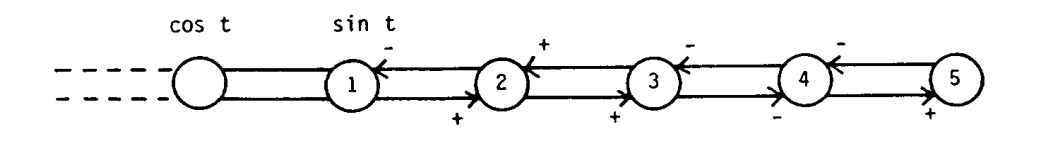
\includegraphics[height=2.0cm]{figure2.png}
	\caption{An illustration of the idea of the proof of Lemma 2. Attachment of a staright chain with node set $\{2,3,4,5\}$ to subsystem at node 1.} 
\end{figure}

\begin{example}
	
%	Consider a example with matrix A of order 5 which satisfying above property of lemma. Now we have to find $\tilde{A} \in Q(A)$ and strictly sinusoidal x satisfyying $\dot{x}=\tilde{A}x$.
%	To find we use above algorithm of proof.  Consider attachment of a straight chain with node set $\{2,3,\ldots, 5\}$ to a subsystem with strictly sinusoidal node values at node 1. Assume node 1 has the value $\sin t$.
%	So,
%	\begin{center}
%		$\tilde{A}=$
%		$\begin{bmatrix}
%			0& a_{12} & 0& 0 &0\\
%			a_{21}& 0& a_{23} & 0& 0\\
%			0 & a_{32}& 0 & a_{34}& 0\\
%			0& 0 & a_{43}& 0 & a_{45}\\
%			0 &0 &0 &a_{54} & 0
%		\end{bmatrix}$
%	\end{center}
%	Now, Solving the system  $\dot{x} = \tilde{A}x$, so
%	\begin{center}
%		$\begin{bmatrix}
%			0& a_{12} & 0& 0 &0\\
%			a_{21}& 0& a_{23} & 0& 0\\
%			0 & a_{32}& 0&  a_{34}& 0\\
%			0& 0 & a_{43}& 0 & a_{45}\\
%			0 &0 &0 &a_{54} & 0
%		\end{bmatrix}$
%	 $\begin{bmatrix}
%	 	x_1 \\
%	 	x_2 \\
%	 	x_3 \\
%	 	x_4 \\
%	 	\sin t \\
%	 \end{bmatrix}$
%	 =
%	 $\begin{bmatrix}
%	 	\dot{x_1} \\
%	 	\dot{x_2}\\
%	 	\dot{x_3}\\
%	 	\dot{x_4}\\
%	 	\cos t \\
%	 \end{bmatrix}$
%	\end{center}
%
%  Equating the row fifth equation we get $a_{54}x_4=\cos t$.By the algorithm of the proof let tentatively set $a_{54}=1$ we get $x_4=\cos t$.
%  
%  Again solving the row 4 equation we get $a_{43}x_3 +a_{45} \sin t= -\sin t$. So,let node value of node 3 is $\sin t$ so choose $a_{43} =-1$ and $a_{45} =-2$ to satisfy equation.
%  
%  Similarly doing for node 3, equating the equation at row 3, we get  $a_{32}x_2 +a_{34} \cos t= -\cos t$. So, let node value of node 2 is $-\cos t$ so choose $a_{32} =1$ and $a_{34} =2$ to satisfy equation.
%  
%  Again solving the row 2 equation we get $a_{21}x_1 +a_{23} \sin t= \sin t$. So,let node value of node 1 is $\sin t$ so choose $a_{21} =1/2$ and $a_{23} =1/2$ to satisfy equation.
%  
%  Lastly solving for row 1 equation, we get $a_{12}(-\cos t) = \cos t$ so choose $a_{12}=-1$ to satisfy row equation. Hence we get,
%  \begin{center}
%  	$\tilde{A}=$
%  	$\begin{bmatrix}
%  		0& -1 & 0& 0 &0\\
%  		1/2& 0& 1/2 & 0& 0\\
%  		0 & 1 & 0& 2 & 0\\
%  		0& 0 & 1& 0 & -2\\
%  		0 &0 &0 &1 & 0
%  	\end{bmatrix}$
%  and $x=$
%   $\begin{bmatrix}
%  	\sin t \\
%  	-\cos t \\
%  	\sin t \\
%  	\cos t \\
%  	\sin t \\
%  \end{bmatrix}$
%  \end{center}
%and satisfying equation;
% \begin{center}
%
%	$\begin{bmatrix}
%		0& -1 & 0& 0 &0\\
%		1/2& 0& 1/2 & 0& 0\\
%		0 & 1 & 0& 2 & 0\\
%		0& 0 & 1& 0 & -2\\
%		0 &0 &0 &1 & 0
%	\end{bmatrix}$
%	$\begin{bmatrix}
%		\sin t \\
%		-\cos t \\
%		\sin t \\
%		\cos t \\
%		\sin t \\
%	\end{bmatrix}$
% =
%$\begin{bmatrix}
%	\cos t \\
%	\sin t\\
%	\cos t\\
%	-\sin t\\
%	\cos t \\
%\end{bmatrix}$
%\end{center}

Consider an example with matrix $A$ of order 5 that satisfies the property of the lemma. Our goal is to find $\tilde{A} \in Q(A)$ and a strictly sinusoidal vector $x$ satisfying $\dot{x}=\tilde{A}x$. To achieve this, we employ the algorithm outlined in the proof.

Let's start by attaching a straight chain with node set $\{2,3,\ldots, 5\}$ to a subsystem with strictly sinusoidal node values at node 1, where node 1 has the value $\sin t$. We represent $\tilde{A}$ as:

\[
\tilde{A} = 
\begin{bmatrix}
	0 & a_{12} & 0 & 0 & 0 \\
	a_{21} & 0 & a_{23} & 0 & 0 \\
	0 & a_{32} & 0 & a_{34} & 0 \\
	0 & 0 & a_{43} & 0 & a_{45} \\
	0 & 0 & 0 & a_{54} & 0
\end{bmatrix}
\]

Solving the system $\dot{x} = \tilde{A}x$, we have:

\[
\begin{bmatrix}
	0 & a_{12} & 0 & 0 & 0 \\
	a_{21} & 0 & a_{23} & 0 & 0 \\
	0 & a_{32} & 0 & a_{34} & 0 \\
	0 & 0 & a_{43} & 0 & a_{45} \\
	0 & 0 & 0 & a_{54} & 0
\end{bmatrix}
\begin{bmatrix}
	x_1 \\
	x_2 \\
	x_3 \\
	x_4 \\
	\sin t
\end{bmatrix}
=
\begin{bmatrix}
	\dot{x_1} \\
	\dot{x_2} \\
	\dot{x_3} \\
	\dot{x_4} \\
	\cos t
\end{bmatrix}
\]

Equating the fifth row equation, we find $a_{54}x_4=\cos t$. Setting $a_{54}=1$, we obtain $x_4=\cos t$. 

Solving the row 4 equation yields $a_{43}x_3 + a_{45} \sin t = -\sin t$. Choosing the node value of node 3 is $\sin t$, we choose $a_{43} = -1$ and $a_{45} = -2$ to satisfy the equation.


Similarly, we solve the row 3 equation by equating it to $a_{32}x_2 +a_{34} \cos t= -\cos t$. Choosing the node value of node 2 to be $-\cos t$, we set $a_{32} = 1$ and $a_{34} = 2$ to satisfy the equation.

Continuing, we solve the row 2 equation by setting it equal to $a_{21}x_1 +a_{23} \sin t= \sin t$. We choose the node value of node 1 as $\sin t$, thus we set $a_{21} = 1/2$ and $a_{23} = 1/2$ to satisfy the equation.

Finally, solving the row 1 equation, we have $a_{12}(-\cos t) = \cos t$. To satisfy this equation, we set $a_{12}=-1$.

 Hence, after completing all the steps, we obtain:
\begin{center}
	$\tilde{A}=
	\begin{bmatrix}
		0 & -1 & 0 & 0 & 0 \\
		1/2 & 0 & 1/2 & 0 & 0 \\
		0 & 1 & 0 & 2 & 0 \\
		0 & 0 & 1 & 0 & -2 \\
		0 & 0 & 0 & 1 & 0
	\end{bmatrix}$
	and $x=
	\begin{bmatrix}
		\sin t \\
		-\cos t \\
		\sin t \\
		\cos t \\
		\sin t
	\end{bmatrix}$
\end{center}

This $\tilde{A}$ and $x$ combination satisfies the equation;
 \begin{center}
		$\begin{bmatrix}
				0& -1 & 0& 0 &0\\
				1/2& 0& 1/2 & 0& 0\\
				0 & 1 & 0& 2 & 0\\
				0& 0 & 1& 0 & -2\\
				0 &0 &0 &1 & 0
			\end{bmatrix}$
		$\begin{bmatrix}
				\sin t \\
				-\cos t \\
				\sin t \\
				\cos t \\
				\sin t \\
			\end{bmatrix}$
	 =
	$\begin{bmatrix}
			\cos t \\
			\sin t\\
			\cos t\\
			-\sin t\\
			\cos t \\
		\end{bmatrix}$
		\end{center}
\end{example}

\begin{thm}
	Suppose $A$ is irreducible and $SD(A)$ has no $k$-cycle, $k > 2$. If there exists a strictly sinusoidal trajectory $x$ solving $\dot{x} = \tilde{A}x$ for some $\tilde{A} \in Q(A)$ then $SD(A)$ has at least one negative 2-cycle and $SD(A)$ is not $\lambda$-consistent.
\end{thm}


\begin{proof}

	Suppose we have a matrix $\tilde{A}$ that belongs to the qualitative class of $A$, denoted as $Q(A)$, along with a strictly sinusoidal trajectory $x$ characterized by certain constants ${\lambda_j}$. Let's assume there exists a 1-cycle at node $i$ within the system. Now, consider the quantity $\Lambda$, defined as $\Lambda = \sum_{i=1}^n \lambda_i x_i^2/2$. for all nodes $i$.
	
	If the signed digraph $SD(A)$ were to be $\lambda$-consistent, then along the trajectory $x$, the derivative of $\Lambda$ would be calculated as $\dot{\Lambda} = \sum_{i=1}^n \lambda_i\tilde{a_{ii}} x_i^2$, which must be greater than zero. However, this contradicts the periodicity property, where $\Lambda(x(t))$ is equal to $\Lambda(x(t+2\pi))$. Lemma 1 concludes that $SD(A)$ must indeed contain a negative 2-cycle.
	
\end{proof}

\begin{cor}
	If $A$ is irreducible and $SD(A)$ has no $k$-cycle, $k > 2$, and exactly one 1-cycle, then no $\tilde{A} \in Q(A)$ admits a strictly sinusoidal trajectory.
\end{cor}

\begin{proof}
	Given these conditions, $SD(A)$ is $\lambda$-consistent, as per Theorem 3.1.5, which effectively rules out the existence of a strictly sinusoidal trajectory.
\end{proof}
